\begin{figure}[h]
\centering
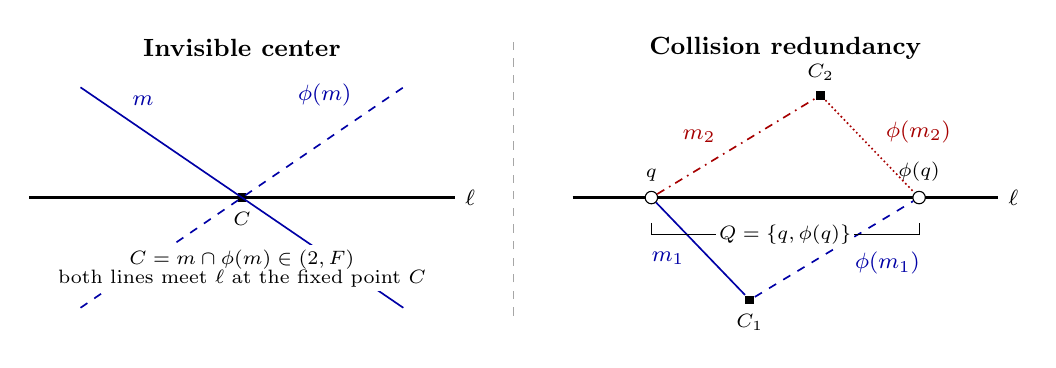
\begin{tikzpicture}[
  x=1cm,y=1cm,
  every node/.style={font=\footnotesize},
  carrier/.style={very thick},
  first/.style={semithick,blue!65!black},
  firstphi/.style={semithick,blue!65!black,dashed},
  second/.style={semithick,red!65!black,dash dot},
  secondphi/.style={semithick,red!65!black,densely dotted},
  fixed/.style={rectangle,fill=black,minimum size=3.2pt,inner sep=0pt},
  candidate/.style={circle,draw,fill=white,minimum size=4.5pt,inner sep=0pt}
]
  \begin{scope}
    \node[font=\small\bfseries] at (2.7,3.05) {Invisible center};
    \draw[carrier] (0,1.15) -- (5.4,1.15)
      node[right] {$\ell$};
    \node[fixed,label={[font=\scriptsize]below:$C$}] (c) at (2.7,1.15) {};
    \draw[first] (0.65,2.55) -- (4.75,-0.25)
      node[pos=0.13,above right] {$m$};
    \draw[firstphi] (0.65,-0.25) -- (4.75,2.55)
      node[pos=0.87,above left] {$\phi(m)$};
    \node[align=center,font=\scriptsize,fill=white,inner sep=1.5pt] at (2.7,0.25)
      {$C=m\cap\phi(m)\in\PG(2,F)$\\[-1pt]
       both lines meet $\ell$ at the fixed point $C$};
  \end{scope}

  \draw[dashed,black!35] (6.15,-0.35) -- (6.15,3.2);

  \begin{scope}[xshift=6.9cm]
    \node[font=\small\bfseries] at (2.7,3.05) {Collision redundancy};
    \draw[carrier] (0,1.15) -- (5.4,1.15)
      node[right] {$\ell$};
    \node[candidate,label={[font=\scriptsize]above:$q$}] (q) at (1.0,1.15) {};
    \node[candidate,label={[font=\scriptsize]above:$\phi(q)$}] (qp) at (4.4,1.15) {};

    \node[fixed,label={[font=\scriptsize]below:$C_1$}] (c1) at (2.25,-0.15) {};
    \node[fixed,label={[font=\scriptsize]above:$C_2$}] (c2) at (3.15,2.45) {};
    \draw[first] (q) -- (c1) node[pos=0.43,below left] {$m_1$};
    \draw[firstphi] (c1) -- (qp)
      node[pos=0.57,below right] {$\phi(m_1)$};
    \draw[second] (q) -- (c2) node[pos=0.43,above left] {$m_2$};
    \draw[secondphi] (c2) -- (qp)
      node[pos=0.57,above right] {$\phi(m_2)$};
    \draw[thin] (1.0,0.83) -- (1.0,0.68) -- (4.4,0.68) -- (4.4,0.83);
    \node[font=\scriptsize,fill=white,inner sep=1pt] at (2.7,0.68)
      {$Q=\{q,\phi(q)\}$};
  \end{scope}
\end{tikzpicture}
\caption{The two corrections to the first-order obstruction count on an
empty fixed carrier \(\ell\).  Left: when the fixed center
\(C=m\cap\phi(m)\) lies on \(\ell\), the conjugate secants meet the carrier
only at a fixed point and charge no candidate pair.  Right: two distinct
visible secant orbits have different fixed centers but charge the same
candidate \(Q=\{q,\phi(q)\}\); only one forbidden pair remains in the
support.  Solid/dashed and dash-dot/dotted lines distinguish the conjugate
secants in the two visible orbits.}
\label{fig:mate-line-correction}
\end{figure}
